Supervised machine learning assumes that training and testing data are sampled from the same distribution, while in practice, the training and testing data are typically collected from related domains but under different distributions, a phenomenon known as domain shift.
However, in real scenarios, it is often prohibitively expensive and time-consuming to acquire a large number of manually annotated labels to retrain a  model for testing data.
An alternative is Unsupervised Domain Adaptation (UDA) \cite{ben2010theory,TransferLearningSurvey} which tackles domain shift by leveraging knowledge learned from the labeled source domain to boost model performance on the unlabeled target domain.


\begin{figure}[H]
    \centering
    \subfloat{
        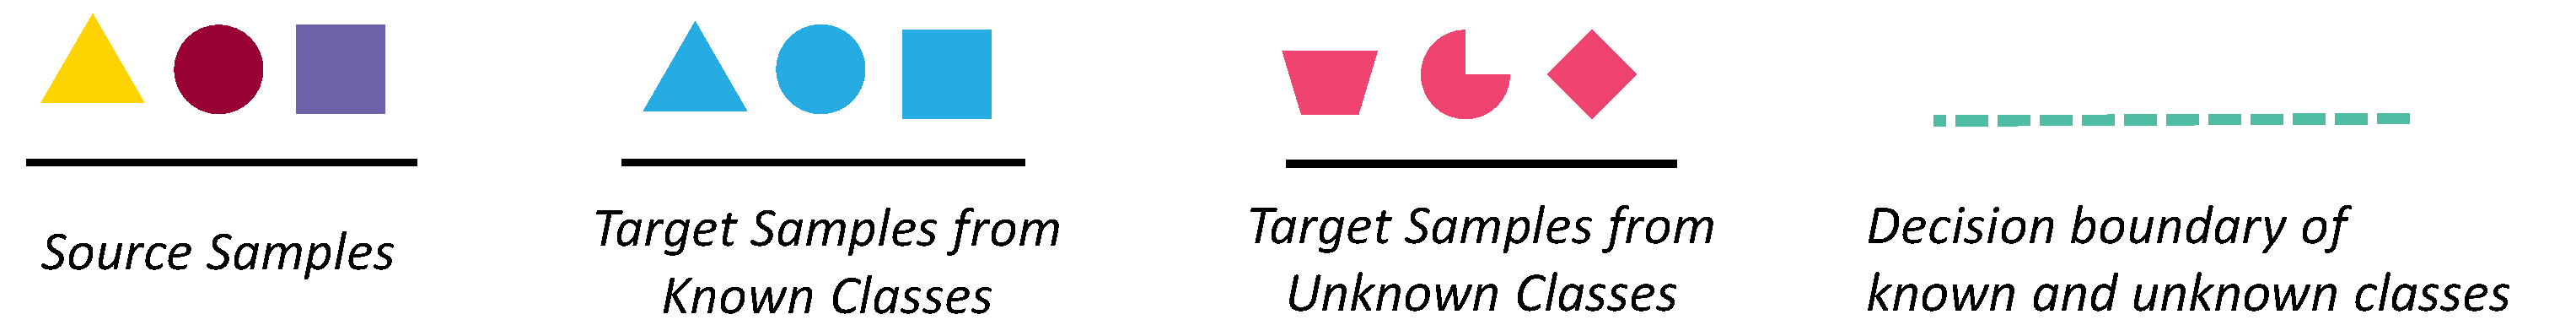
\includegraphics[width=0.55\textwidth]{contents/figures/pdf/overview/note.pdf} 
    }
    \\
    \addtocounter{subfigure}{-1}
    \subfloat[]{
        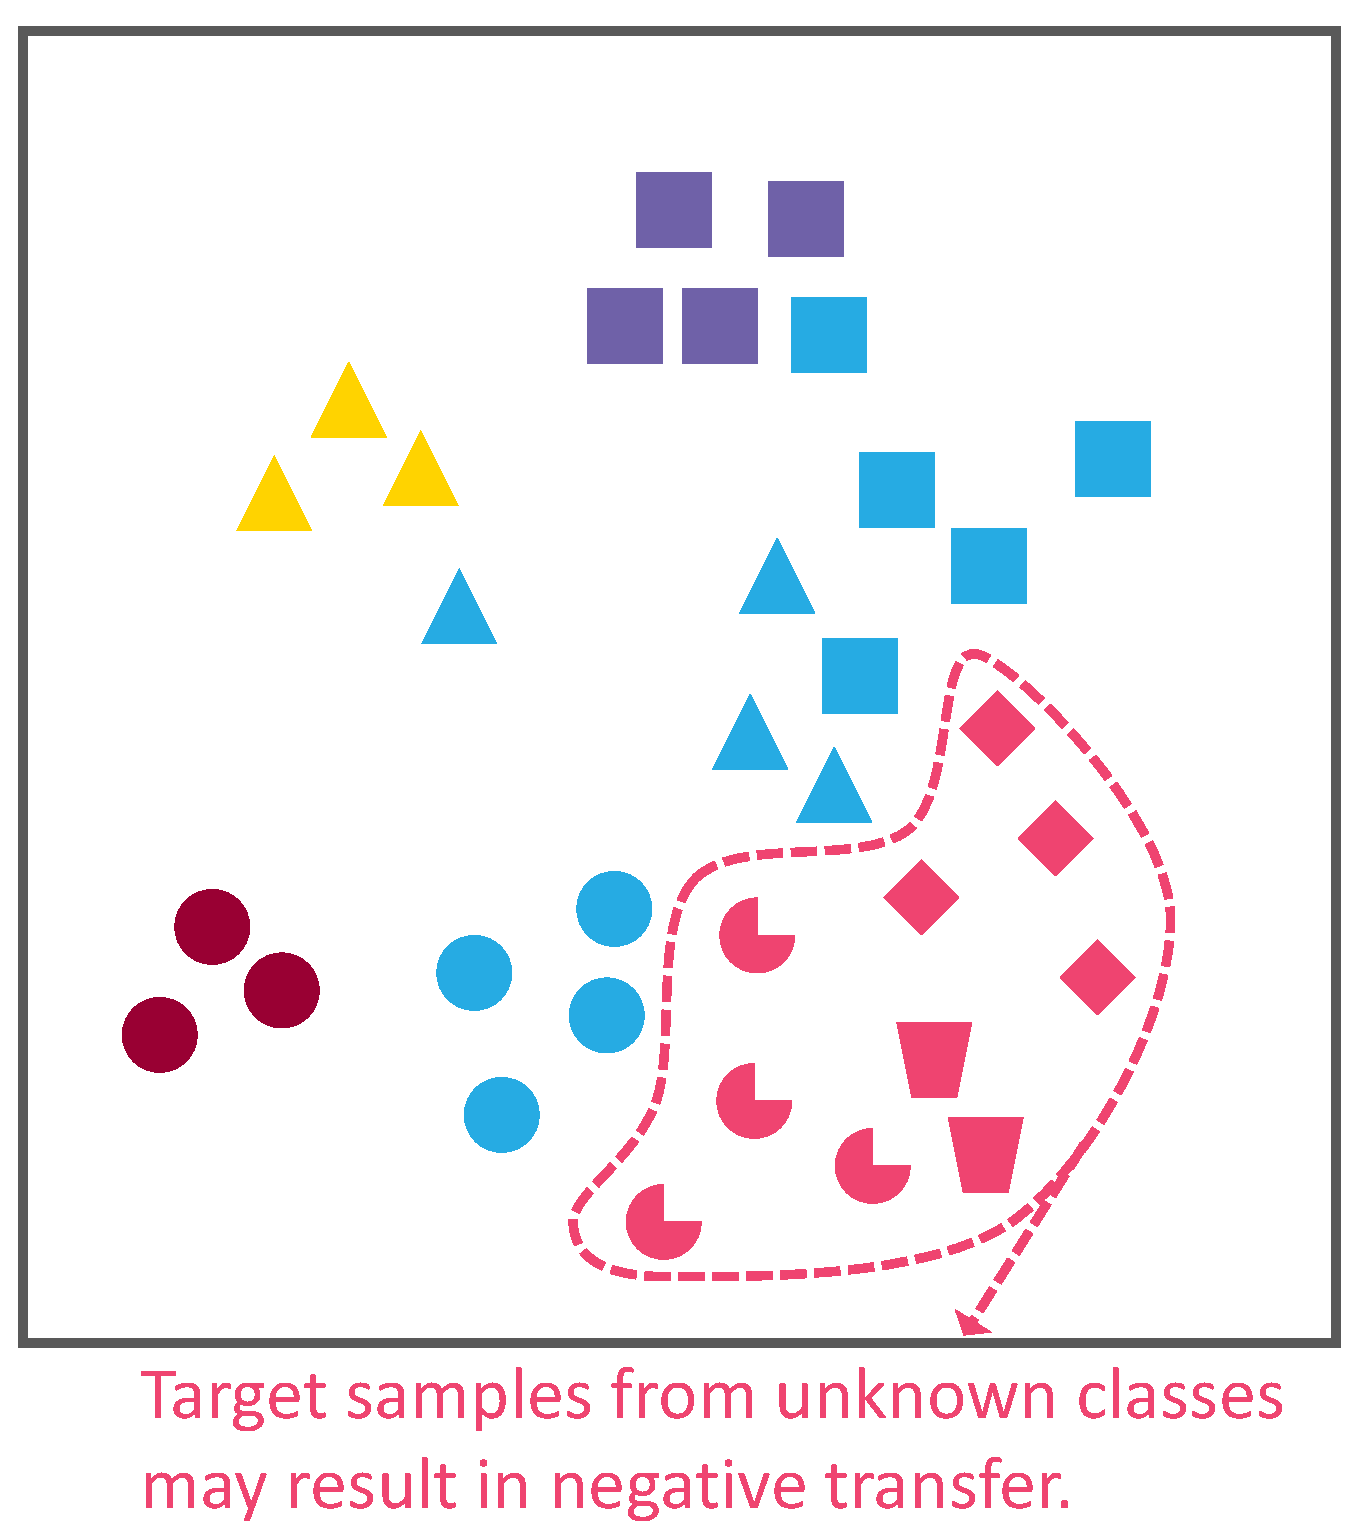
\includegraphics[width=0.22\textwidth]{contents/figures/pdf/overview/1.pdf} 
        \label{figure: reweighting based}
    } 
    \subfloat[]{
        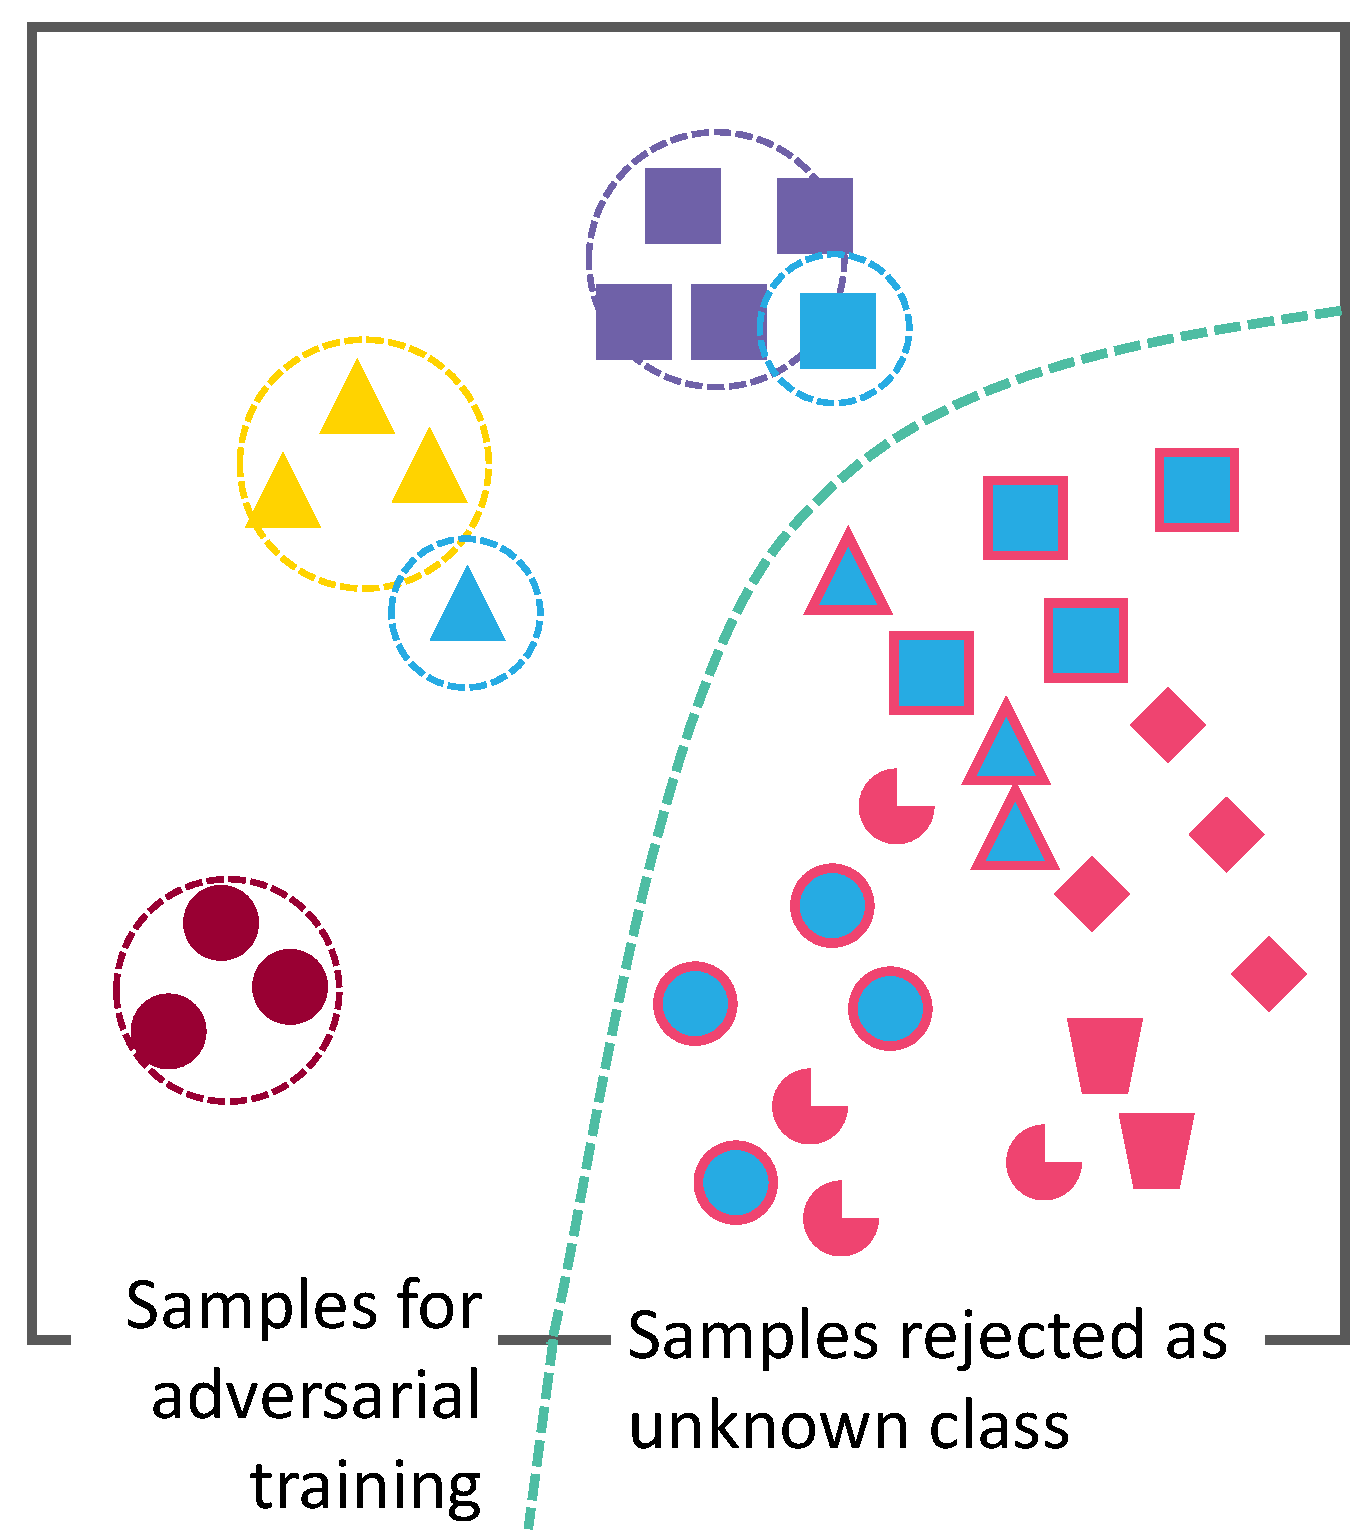
\includegraphics[width=0.22\textwidth]{contents/figures/pdf/overview/2.pdf} 
        \label{figure: ThDAN 1}
    } 
    \subfloat[]{
        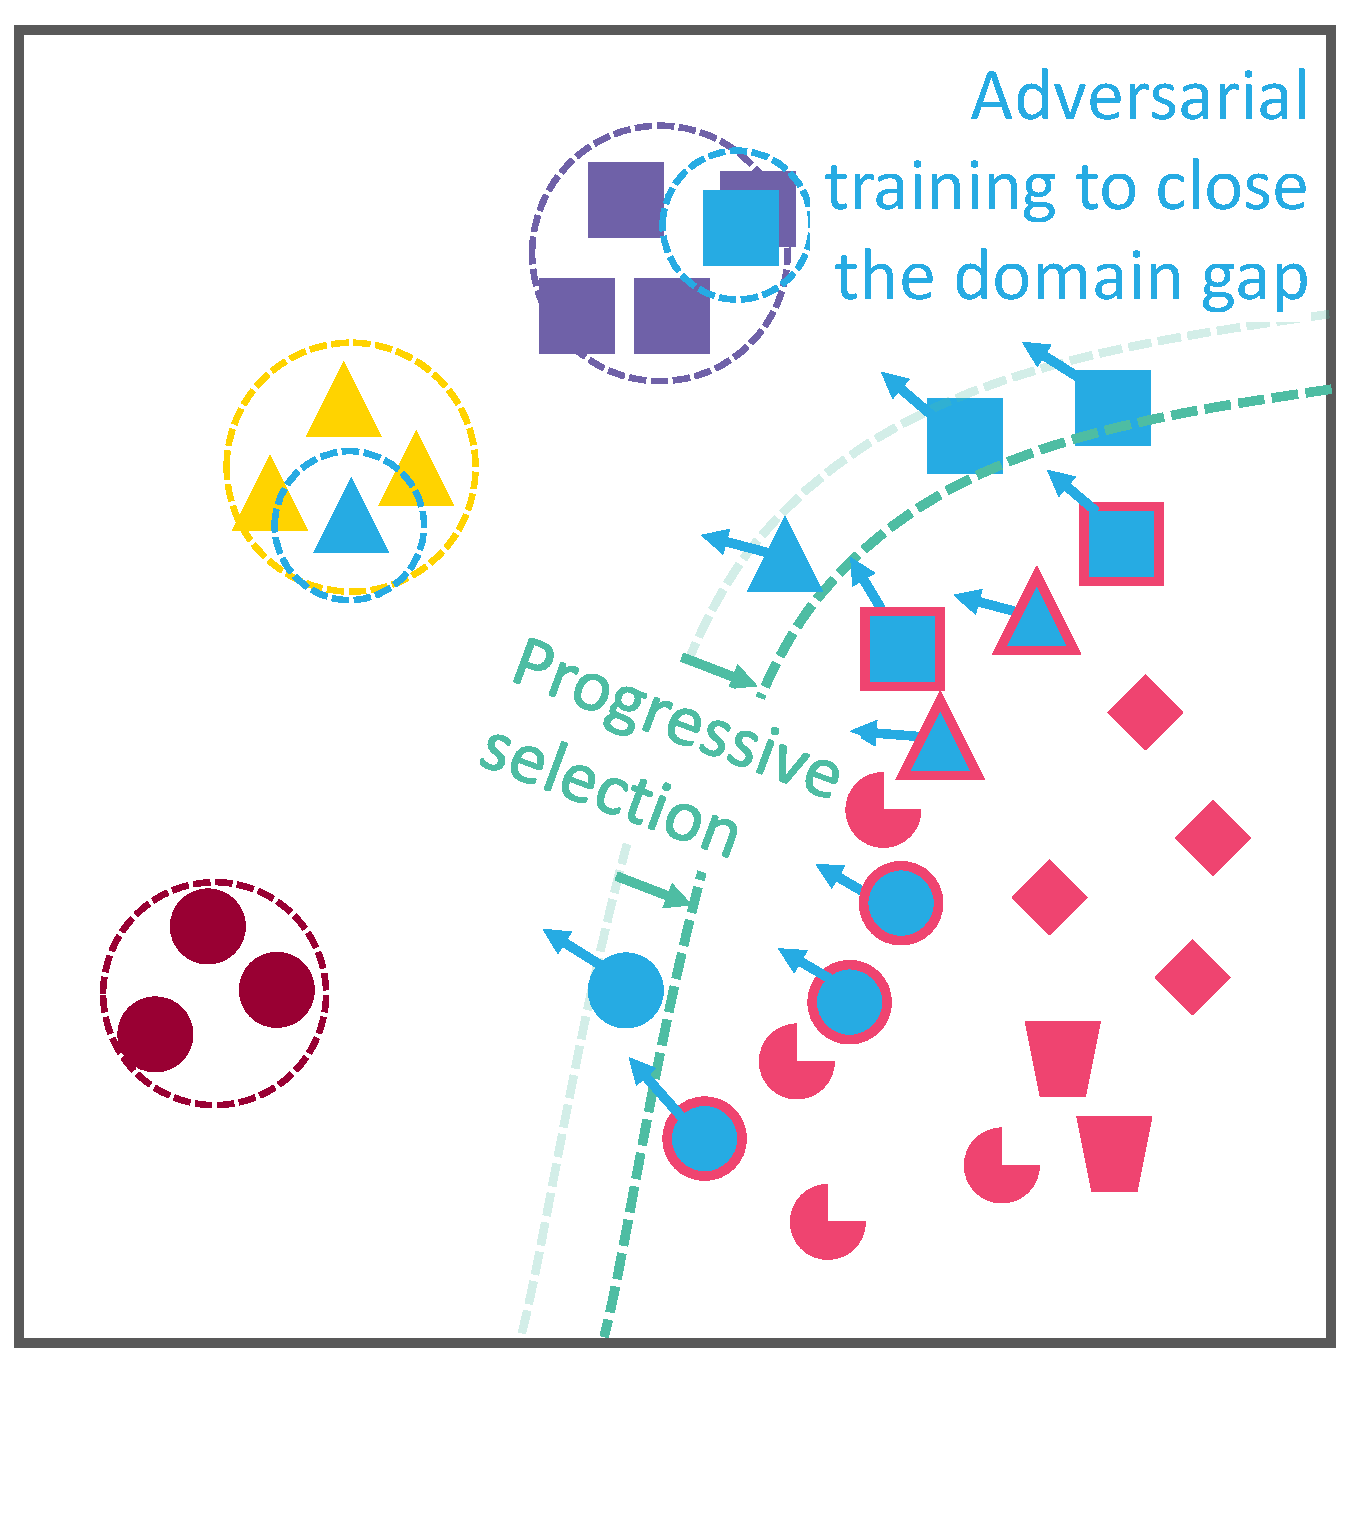
\includegraphics[width=0.22\textwidth]{contents/figures/pdf/overview/3.pdf} 
        \label{figure: ThDAN 2}
    } 
    % \hfil
    \subfloat[]{
        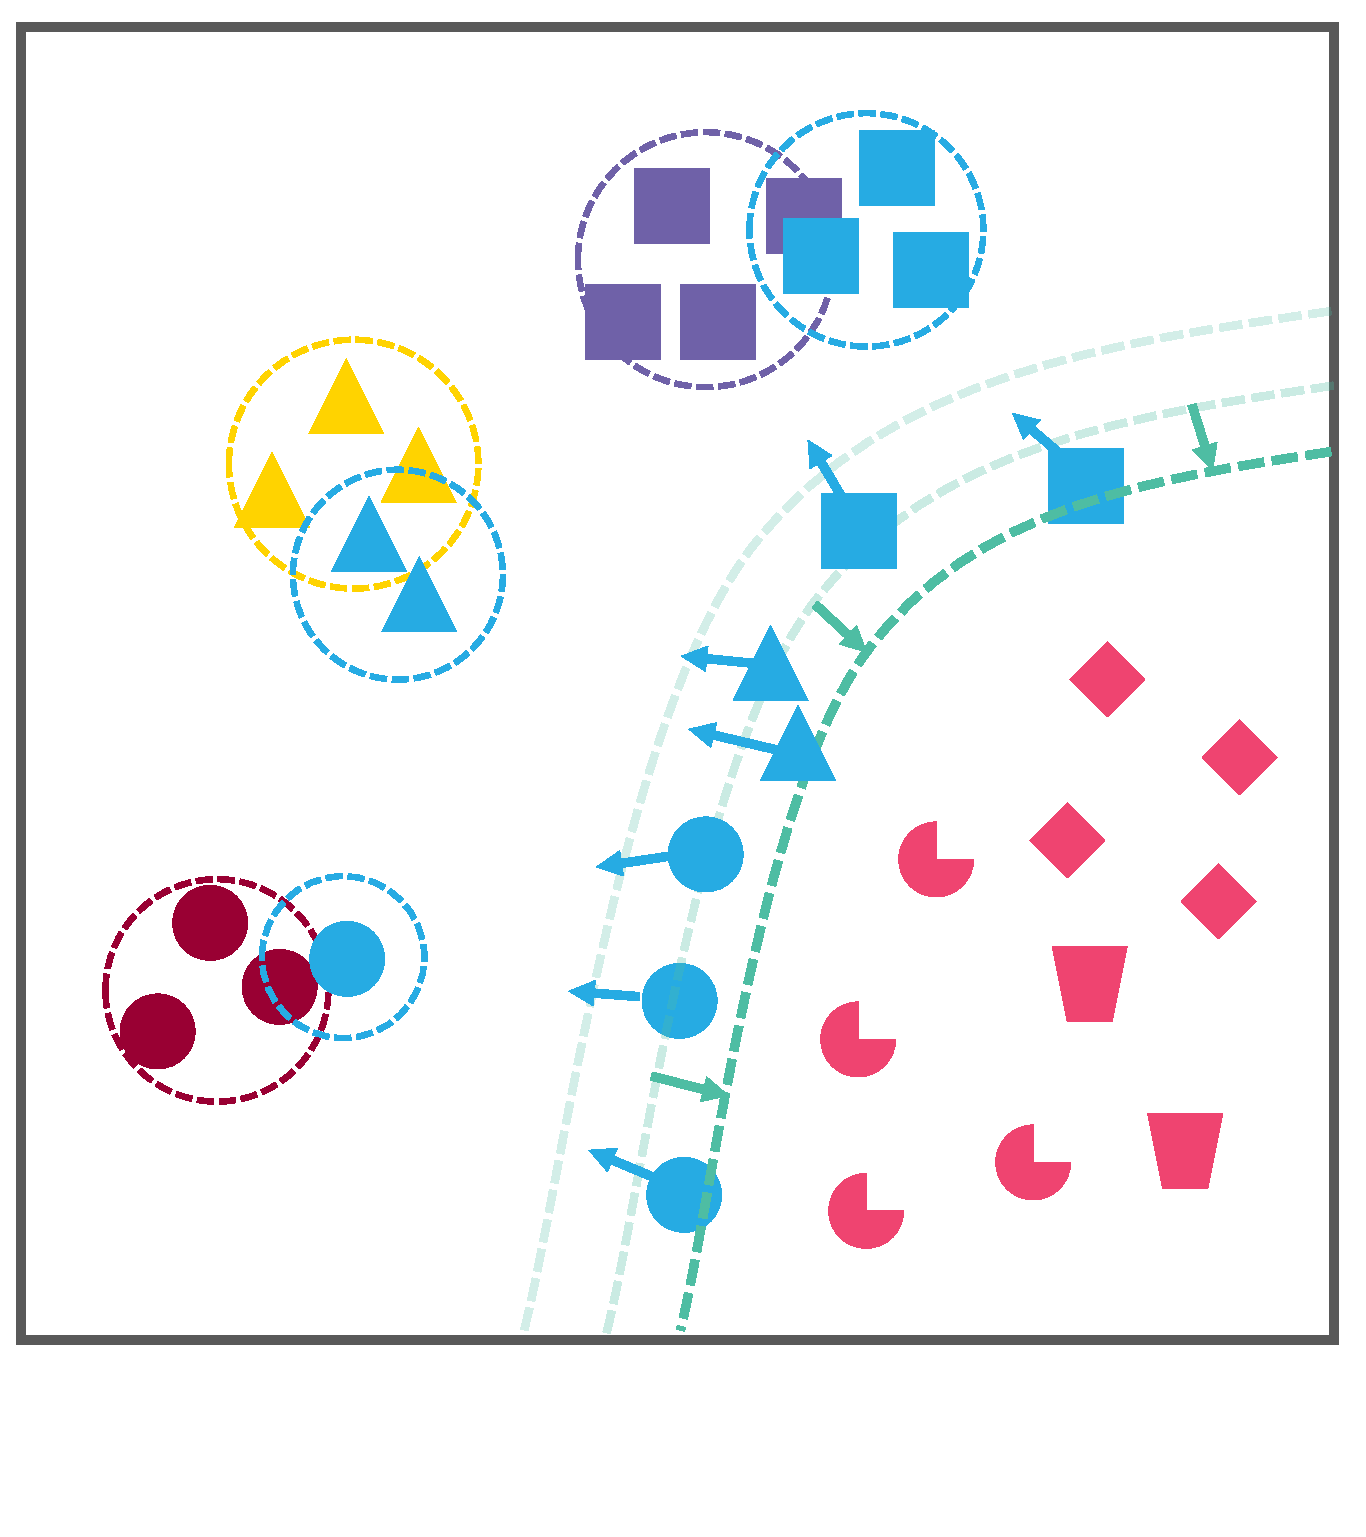
\includegraphics[width=0.22\textwidth]{contents/figures/pdf/overview/4.pdf} 
        \label{figure: ThDAN 3}
    }
    \caption{
        Figure1 of the original manuscript.
    } 
    \label{figure: overview} 
\end{figure}



Over the last decade many UDA methods \cite{DeepDomainConfusion,long2015learning,long2016unsupervised,tao2014sparsity,DomainAdversrialNetwork,liu2018coupled} have been proposed for \textit{Close Set domain adaptation (\textbf{CSDA})}, which assumes the label space of the source and target domain is identical.
However, such assumption can hardly be verified since label information of the target samples is unavailable, especially in real scenarios where we cannot constrain the boundary of classes in the target domain.
A more practical setting is the \textit{Open Set domain adaptation (\textbf{OSDA})}  proposed in \cite{OpensetsDA} where the source and target domain both contain samples that do not belong to the classes of each other.
The objective of OSDA is to categorize the target samples of known classes correctly, and reject the ones of unknown classes as "unknown".
However, collecting source samples of unknown classes is also expensive because we must collect diverse and many samples to obtain the concept of "unknown".
Thus, in this paper, we follow the setting of \cite{OpensetDA-bp} where the unknown source samples are no longer available, \text{i.e}, the label space of target domain contains the label space of source domain.

Domain adversarial training as a proposing way for CSDA transfers knowledge by adversarially aligning distributions of source and target domain.
However, if we apply domain adversarial training for OSDA to align whole feature space would incur the negative transfer since distributions of the target samples from the unknown classes cannot be correctly aligned.
The \textit{Open Set Back-Propagation } model proposed in \cite{OpensetDA-bp} tackles this problem by gradually assigning smaller weights to the samples from unknown classes, so that the negative transfer in OSDA can be alleviated.
However, since the weights of samples from the known and unknown classes are similar in the initial stage, the model would suffer from a serious negative transfer in the beginning.
Moreover, because all the samples from the unknown class are used for training, the model would need a longer time to reduce the negative influence caused by them.

To overcome the limitations of existing method for OSDA, this paper presents a \textit{Thresholded Domain Adversarial Network (\textbf{ThDAN})}, which progressively selects transferable target samples for domain adversarial training. 
\figurename{\ref{figure: overview}} illustrated the general idea of ThDAN.
Based on the fact that samples from the known classes is more transferable than target samples of the unknown ones, we derive a criterion to quantify the transferability by constructing classifiers to categorize known classes and to discriminate unknown class.
By averaging transferability scores of source domain samples, a \textit{transferability threshold} is adaptively computed to select transferable samples, the procedure of sample selection is illustrated in \figurename{\ref{figure: selection}}.
Then, as shown in \figurename{\ref{figure: ThDANN}}, the proposed ThDAN will be trained to reject unselected samples as "unknown" and generate domain-invariant features between the selected samples and the source samples via a gradient reversal layer \cite{DomainAdversrialNetwork}, by this mean, our model can better solve the OSDA problem.
Moreover, to make the sample selection algorithm robust to the oscillation of mini-batch training and the continuous-changing of domain gap, we perform Progressive Sample Selection for ThDAN, at each iteration, the transferability threshold is tweaked to select more target samples from the known classes for adversarial training.

In summary, our contributions are as follows,

\begin{itemize}

    \item A novel model namely \textit{Thresholded Domain Adversarial Network (\textbf{ThDAN})} is proposed for Open Set Domain Adaptation by selecting transferable target samples for domain adversarial training.

    \item We propose a \textit{Progressive Sample Selection} strategy for ThDAN by progressively tweaking the transferability threshold during the training process.

    \item Comprehensive experiments demonstrate that the proposed method outperforms state-of-the-art close set, open set domain adaptation and open set recognition approaches on three benchmarks.

\end{itemize}



